\documentclass[10pt,a4paper]{article}

\usepackage[utf8]{inputenc}
\usepackage[T1]{fontenc}
\usepackage[indonesian]{babel}
\usepackage[a4paper,top=2cm,bottom=2cm,left=2cm,right=2cm]{geometry}
\usepackage{xcolor}
\usepackage{titlesec}
\usepackage{graphicx}
\graphicspath{{figures/}}
\usepackage{booktabs}
\usepackage{tabularx}
\usepackage{enumitem}
\usepackage{placeins}
\usepackage{amsmath}
\usepackage{parskip}
\usepackage[hidelinks]{hyperref}

\titleformat{\section}{\large\bfseries}{\thesection.}{0.5em}{}
\titleformat{\subsection}{\normalsize\bfseries}{\thesubsection}{0.5em}{}
\titlespacing*{\section}{0pt}{0.8em}{0.3em}
\titlespacing*{\subsection}{0pt}{0.6em}{0.2em}

\setlength{\parindent}{0pt}
\setlength{\parskip}{0.35em}
\setlist{leftmargin=1.6em,itemsep=0.1em,topsep=0.2em}

\begin{document}

\sloppy

% ===================== KOP =====================
\begin{center}
  {\Large\bfseries Write-Up Tugas Besar}\\[0.3em]
  {\Large\bfseries Machine Learning from Scratch pada Kompetisi Kaggle}\\[0.2em]
  {\normalsize AI Lab Recruitment Task 2 (ai-lab-recruitment-task-2)}\\[0.5em]
  \rule{0.85\textwidth}{0.6pt}\\[0.6em]
  \begin{tabularx}{0.6\textwidth}{|l|X|}
    \hline
    \textbf{Nama} & Kurt Mikhael Purba \\
    \hline
    \textbf{NIM} & 13524065 \\
    \hline
  \end{tabularx}
\end{center}

\section{TLDR}

 Write-up ini mendokumentasikan proses implementasi Decision Tree Learning, Logistic Regression, dan SVM dari nol dengan NumPy untuk kompetisi klasifikasi tabular di Kaggle. Ketiga model dibandingkan dengan implementasi scikit-learn dan digunakan untuk menghasilkan beberapa submisi. Target yang diprediksi adalah \texttt{loan\_status} dengan metrik macro F1. Proses eksperimen berlangsung dalam empat tahap notebook, yaitu v1 sampai v4. Tahap pertama (v1) membangun pipeline robust dengan repeated stratified 5-fold cross-validation, tuning threshold exact untuk macro F1, dan feature expansion tanpa bocor ke test. Tahap kedua (v2) menambahkan CART cost-sensitive dengan bobot kelas positif di dalam Gini impurity. Tahap ketiga (v3) menguji eksperimen terkontrol dengan memasukkan \texttt{person\_id} sebagai fitur setelah audit train-only menunjukkan struktur source-order yang kuat. Tahap keempat (v4) memperluas pencarian CART ID-aware ke leaf yang lebih kecil dan memilih model berdasarkan stabilitas Macro-F1 serta threshold pada repeated OOF. Submisi publik terbaik yang tercatat adalah \texttt{submission\_best\_scratch\_v4.csv} dengan skor 0.89837, diikuti 0.88735 (submisi ID-aware v2-plus), 0.86571 (weighted CART), 0.85409 (CART robust), dan 0.84573 (baseline pertama).

\section{Problem Overview}

Kompetisinya adalah \emph{AI Lab Recruitment Task 2}, klasifikasi biner tabular untuk kelayakan pinjaman. Setiap baris berisi karakteristik pemohon seperti \texttt{person\_age}, \texttt{person\_income}, \texttt{person\_home\_ownership}, \texttt{person\_emp\_length}, \texttt{loan\_amnt}, \texttt{loan\_int\_rate}, \texttt{loan\_percent\_income}, \texttt{credit\_score}, dan \texttt{previous\_loan\_defaults\_on\_file}. Targetnya \texttt{loan\_status} bernilai 0 atau 1 dengan kelas positif sebagai minoritas. Kompetisi memakai macro F1, rata rata F1 kelas 0 dan kelas 1, jadi performa di kelas mayoritas saja tidak cukup.

Aturannya tegas. Ketiga algoritma harus from scratch dan hanya boleh memakai library komputasi matematis seperti NumPy. Pandas hanya untuk membaca tabel, matplotlib untuk visualisasi, dan scikit-learn hanya sebagai pembanding sekaligus penyedia metrik. Tidak boleh ada ensemble method atau algoritma di luar yang disebutkan untuk submisi. File submisi harus berisi \texttt{person\_id} dan \texttt{loan\_status} dengan urutan identik terhadap test.

\subsection{Data dan Preprocessing}

Dataset terdiri dari data train berlabel, data test tanpa label, dan template submisi. Kolom
\texttt{loan\_status} hanya digunakan sebagai target pada train, sedangkan \texttt{person\_id}
disimpan terpisah sebagai identifier untuk menjaga urutan submisi. Fitur kategorikal diubah menjadi
representasi numerik secara manual menggunakan preprocessor scratch, sementara fitur numerik
dinormalisasi menggunakan statistik yang dipelajari dari data train pada fold terkait. Dengan demikian,
statistik preprocessing tidak dihitung dari validation fold atau test.

Pada pipeline utama, fitur yang dipakai tanpa \texttt{person\_id} mencakup fitur demografis,
finansial, dan riwayat kredit. Logistic Regression dan SVM juga diuji dengan feature expansion
berbasis quantile serta interaksi kategori yang target-independent. Ekspansi tersebut tetap menjadi
bagian dari preprocessing; model akhirnya tetap Logistic Regression atau linear SVM. Cabang ID-aware
diperlakukan sebagai eksperimen sensitivitas terpisah dan tidak dicampur dengan hasil baseline yang
tidak memakai identifier.

\section{Decision Tree Learning}

Saya memilih CART, bukan ID3 atau C4.5. Alasannya dikarenakan CART menangani fitur numerik kontinu secara alami lewat threshold biner, sedangkan ID3 butuh diskretisasi dan C4.5 menangani multiway split. Selain itu pembanding scikit-learn \texttt{DecisionTreeClassifier} juga berbasis CART, jadi perbandingannya fair.

Implementasi saya menumbuhkan pohon secara rekursif. Pada tiap node, semua kandidat split dicari dengan mengurutkan nilai fitur, lalu mengambil titik tengah di antara dua nilai yang berbeda. Kandidat yang membuat salah satu child lebih kecil dari \texttt{min\_samples\_leaf} dibuang. Split terbaik dipilih dengan memaksimalkan penurunan Gini impurity

\[
G(S)=1-p_0^2-p_1^2,\qquad
\Delta G=G(\text{parent})-\frac{n_L}{n}G(S_L)-\frac{n_R}{n}G(S_R).
\]

Pertumbuhan berhenti ketika kedalaman maksimal tercapai, jumlah sampel kurang dari \texttt{min\_samples\_split}, atau node homogen. Leaf menyimpan probabilitas kelas positif, dan feature importance diakumulasi dari gain dikali bobot sampel node. Pada versi awal saya membatasi jumlah kandidat threshold (48) agar cepat, tetapi di v1 saya ganti dengan exact search karena kualitas split naik meski waktu training bertambah.

Versi kedua menambahkan weighted Gini. Perhatikan bahwa Macro F1 menghukum kelas minoritas sehingga bobot kelas positif diikutkan dalam perhitungan impurity dan estimasi probabilitas leaf. Parameter \texttt{positive\_class\_weight} ini dituning dari train saja lewat OOF CV, bukan dari leaderboard. Ini tetap satu pohon tunggal, bukan ensemble, jadi tidak melanggar aturan. Perbandingan dengan \texttt{DecisionTreeClassifier} scikit-learn pada split validasi yang sama memberikan pola yang mirip, dan saya tidak menemukan anomali besar antara keduanya.

\section{Logistic Regression}

Logistic Regression dari scratch memakai sigmoid untuk menghasilkan probabilitas kelas positif,

\[
\hat{p}=\sigma(Xw+b)=\frac{1}{1+e^{-(Xw+b)}},
\]

dengan objective weighted binary cross-entropy plus regularisasi L2. Kelas minoritas diberi bobot seimbang yang dihitung manual. Optimisasinya memakai mini-batch dengan optimizer Adam, yang nanti saya jelaskan lebih dalam di bagian bonus. Ada early stopping berbasis patience terhadap loss penuh per epoch, dan saya mencatat loss history untuk visualisasi proses training.

Di v1, model linear mendapat bantuan berupa nonlinear feature expansion yang target-independent. Basis threshold berasal dari quantile pada fitur kunci seperti \texttt{loan\_percent\_income}, \texttt{loan\_int\_rate}, dan \texttt{credit\_score}, plus interaksi dengan \texttt{person\_home\_ownership}. Transformasi ini bukan model baru, prediktor akhirnya tetap Logistic Regression, dan cut-point quantile selalu dipelajari dari training fold saja.

\section{Support Vector Machine}

SVM saya buat sebagai linear SVM dengan label $+1/-1$ dan objective hinge loss plus regularisasi,

\[
\frac{\lambda}{2}\lVert w\rVert^2+\frac{1}{n}\sum_i \max(0,1-y_i(w^Tx_i+b)).
\]

Optimisasi memakai mini-batch subgradient descent dengan learning rate yang menurun seiring epoch. Gradien hanya menerima kontribusi dari observasi yang marginnya di bawah satu. Kelas yang tidak seimbang ditangani dengan sample weight, dan prediksi diambil dari tanda \texttt{decision\_function}. Saya membandingkannya dengan \texttt{LinearSVC} scikit-learn pada preprocessing yang identik.

Perhatikan juga bahwa SVM saya linear sehingga performanya di data yang tidak linear kalah dibanding CART dan feature expansion yang sama seperti LR tidak cukup mengejar. Di akhir, SVM tidak dipakai untuk submisi utama, tapi tetap dipertahankan sebagai implementasi wajib dan pembanding.

\section{Validation Strategy}

Strategi validasi naik bertahap. Baseline awal memakai stratified holdout 80/20 yang diimplementasikan sendiri di NumPy. Setelah itu saya beralih ke repeated stratified 5-fold cross-validation dengan prediksi out-of-fold (OOF). Preprocessing selalu di-fit ulang di dalam setiap fold agar tidak bocor, dan semua keputusan hyperparameter serta threshold hanya melihat train.csv.

Macro F1 sensitif terhadap threshold. Threshold default 0.5 untuk LR dan 0.0 untuk SVM tidak selalu optimal, apalagi dengan kelas tidak seimbang. Saya menulis fungsi exact threshold optimization yang menyortir skor OOF lalu menghitung macro F1 kumulatif dalam $O(n\log n)$, dan memilih threshold yang memaksimalkan macro F1. Dua atau tiga kandidat konfigurasi terbaik dari tuning seed tunggal lalu diuji ulang pada tiga seed CV (42, 2026, 777), dan pemenangnya dipilih dari rata rata repeated OOF macro F1 dengan threshold diambil dari median antar repeat.

Hasil lokal dan leaderboard publik digunakan untuk tujuan yang berbeda. OOF dipakai untuk memilih model,
hyperparameter, dan threshold, sedangkan leaderboard hanya dipakai sebagai evaluasi eksternal setelah
konfigurasi dibekukan. Pada validasi OOF, varian ID-aware CART keluar sebagai kandidat terbaik. V4
membekukan varian tersebut melalui repeated OOF dan menghasilkan
\texttt{submission\_best\_scratch\_v4.csv}. Submission ini memperoleh skor publik 0.89837.
Perbandingan seluruh skor publik yang sudah tercatat ada di
Tabel~\ref{tab:lb}.

Ringkasan perubahan antarversi ditunjukkan pada Tabel~\ref{tab:versions}. Nilai OOF yang tidak
tersimpan sebagai output final notebook sengaja tidak direkonstruksi dari leaderboard.

\begin{table}[h]
\centering
\small
\begin{tabularx}{\textwidth}{l l X X}
\toprule
\textbf{Versi} & \textbf{Fitur} & \textbf{Perubahan utama} & \textbf{Dasar evaluasi} \\
\midrule
v1 & Tanpa \texttt{person\_id} & Pipeline robust, exact CART split, threshold OOF, dan repeated CV & Baseline bebas leakage; skor publik 0.84573 \\
v2 & Tanpa \texttt{person\_id} & Cost-sensitive CART dengan positive-class weight & Skor publik weighted CART 0.86571 \\
v3 & Dengan \texttt{person\_id} & Audit source-order dan eksperimen ID-aware sebagai sensitivity analysis & Skor publik 0.88735 pada submisi v2-plus \\
v4 & Dengan \texttt{person\_id} & Leaf lebih kecil, repeated OOF, dan audit stabilitas threshold & Skor publik 0.89837 pada \texttt{submission\_best\_scratch\_v4.csv} \\
\bottomrule
\end{tabularx}
\caption{Perkembangan pipeline eksperimen dari v1 sampai v4.}
\label{tab:versions}
\end{table}

\begin{table}[h]
\centering
\small
\begin{tabularx}{\textwidth}{lXcc}
\toprule
\textbf{Submisi} & \textbf{Model} & \textbf{Skor Publik} \\
\midrule
submission\_best\_scratch\_v2\_plus.csv & CART scratch dengan person\_id & 0.88735 \\
submission\_best\_scratch\_v4.csv & CART scratch ID-aware, threshold-stable & 0.89837 \\
submission\_best\_scratch\_weighted\_cart\_v2.csv & Weighted CART scratch & 0.86571 \\
submission\_best\_scratch\_robust.csv & CART scratch robust no leakage & 0.85409 \\
submission\_cart\_scratch.csv & CART scratch baseline & 0.84573 \\
\bottomrule
\end{tabularx}
\caption{Skor submisi publik di leaderboard}
\label{tab:lb}
\end{table}

Satu hal yang perlu saya akui di write-up adalah audit train-only di v3 menunjukkan \texttt{person\_id}
membawa struktur urutan yang kuat terhadap target, seperti terlihat di Gambar~\ref{fig:id}. Binning
ID dengan lebar tetap menampilkan positive rate yang melompat antar blok. Eksperimen ID-aware lahir
dari situ sebagai sensitivity analysis. V4 kemudian menghasilkan skor publik tertinggi yang tercatat,
yaitu 0.89837 pada \texttt{submission\_best\_scratch\_v4.csv}, setelah sebelumnya submisi v2-plus
mencapai 0.88735. Peningkatan ini bukan bukti bahwa ID adalah faktor kredit yang sah,
melainkan indikasi bahwa split dataset ini mengandung source-order signal. Tidak ada aturan manual
seperti \texttt{if person\_id > X then 1}; split terhadap ID murni dipelajari sendiri oleh CART.
Generalisasi hasil ini ke data dengan ID yang diacak ulang tidak dapat diasumsikan.

\begin{figure}[h]
\centering
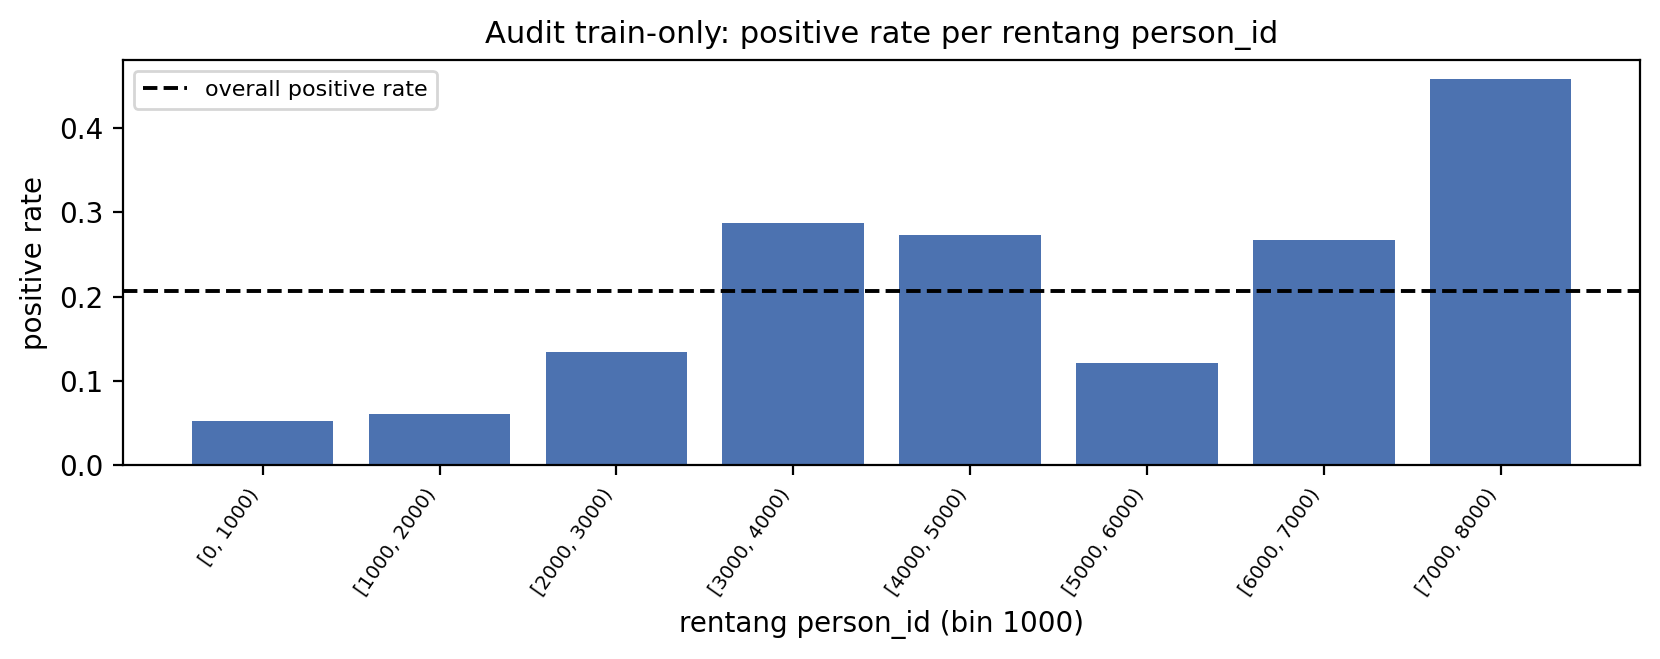
\includegraphics[width=0.92\textwidth]{id_audit_train_only.png}
\caption{Contoh audit train-only - positive rate melompat antar rentang person\_id}
\label{fig:id}
\end{figure}

\section{Percobaan yang Gagal}

Tidak semuanya langsung naik. Beberapa pendekatan yang saya coba gagal atau tidak sesuai harapan.

\begin{enumerate}
\item \textbf{Threshold default dan class weight sekaligus.} Pada versi awal, LR dan SVM memakai balanced class weight lalu tetap di-threshold di 0.5 atau 0.0. Kompensasi kelasnya dobel dan hasilnya tidak optimal. Di versi robust class weight saya matikan dan biarkan threshold OOF yang menangani ketidakseimbangan, hasilnya lebih baik.
\item \textbf{Pembatasan 48 kandidat threshold di CART.} Cepat, tapi split yang ditemukan lebih kasar. Exact search menaikkan skor, jadi subsampling threshold saya buang.
\item \textbf{Pohon dalam tanpa batas.} \texttt{max\_depth=None} tanpa aturan lain membuat pohon overfit. Regularisasi lewat \texttt{min\_samples\_leaf} (40) dan \texttt{min\_samples\_split} (80) yang membuatnya kembali sehat.
\item \textbf{Feature expansion untuk LR dan SVM.} Sudah menaikkan skor, tapi keduanya tetap di bawah CART. Pada akhirnya LR dan SVM tidak pernah menang untuk submisi, walaupun tetap wajib dikerjakan.
\item \textbf{Submisi pertama.} \texttt{submission\_cart\_scratch.csv} dari tahap baseline holdout mendapat 0.84573. Peningkatan berikutnya lahir dari pipeline robust, bukan dari mengubah model dasar.
\end{enumerate}

\section{Pengembangan Lebih Lanjut}

Masih banyak yang bisa dicoba jika waktu tidak terbatas. Saya ingin mencoba SVM nonlinear dengan kernel yang ditulis sendiri di NumPy, misalnya kernel RBF, karena keluarga SVM memang membolehkannya. Selain itu probabilitas leaf CART bisa dikalibrasi dengan Platt scaling atau isotonic regression supaya skor lebih rapi sebelum di-threshold. Ruang tuning \texttt{positive\_class\_weight} dan \texttt{min\_samples\_leaf} bisa diperlebar dengan random search, dan jumlah quantile pada expansion bisa dinaikkan dengan teknik yang lebih hemat memori. Untuk persoalan person\_id, eksperimen permutasi ID bisa mengukur seberapa besar sinyal yang benar benar datang dari urutan data, sehingga kita tahu batas generalisasi model ke data dengan ID teracak.

\section{Bonus}

\subsection{Algoritma Optimasi Tambahan - Adam}

Optimasi tambahan di luar materi kelas yang saya pakai adalah Adam (Kingma dan Ba, 2015), dipakai untuk melatih Logistic Regression dari scratch. Kelas ini biasanya baru mengajarkan gradient descent biasa, dan Adam membedakan diri dengan menjaga estimasi momen pertama dan kedua dari gradien,

\[
m_t=\beta_1 m_{t-1}+(1-\beta_1)g_t,\qquad
v_t=\beta_2 v_{t-1}+(1-\beta_2)g_t^2,
\]

lalu mengoreksi bias karena inisialisasi nol dengan $\hat m_t=m_t/(1-\beta_1^t)$ dan $\hat v_t=v_t/(1-\beta_2^t)$, dan memperbarui parameter dengan

\[
w \leftarrow w-\alpha\frac{\hat m_t}{\sqrt{\hat v_t}+\epsilon}.
\]

Alur kerjanya adalah \texttt{m} menjadi semacam momentum yang meredam osilasi, sedangkan \texttt{v} menormalkan langkah per koordinat sehingga koefisien yang gradiennya besar tidak melompat terlalu jauh dan koefisien yang gradiennya kecil tetap bisa bergerak. Hasilnya konvergensi lebih mulus dan tidak terlalu sensitif terhadap learning rate dibanding SGD polos, dan itulah yang saya amati dari loss history yang turun stabil tanpa bergetar.

\subsection{Gambar Percabangan Tree}

Gambar~\ref{fig:tree} adalah hasil rendering struktur \texttt{tree\_} dari varian CART berbobot
dengan skema fitur yang identik. Karena data kompetisi tidak bisa dibawa keluar dari Kaggle, gambar
ini dibuat dengan menjalankan ulang kelas yang sama pada data dengan skema yang identik agar tetap
dapat direproduksi secara lokal. Pada contoh tersebut, split pertama menggunakan fitur rasio
pendapatan terhadap pinjaman (ditampilkan sebagai \texttt{loan/inc}), kemudian bercabang ke fitur
credit score dan interest rate. Gambar ini merupakan ilustrasi struktur model, bukan klaim bahwa
setiap split tersebut sama persis dengan pohon final ID-aware v4.

\begin{figure}[h]
\centering
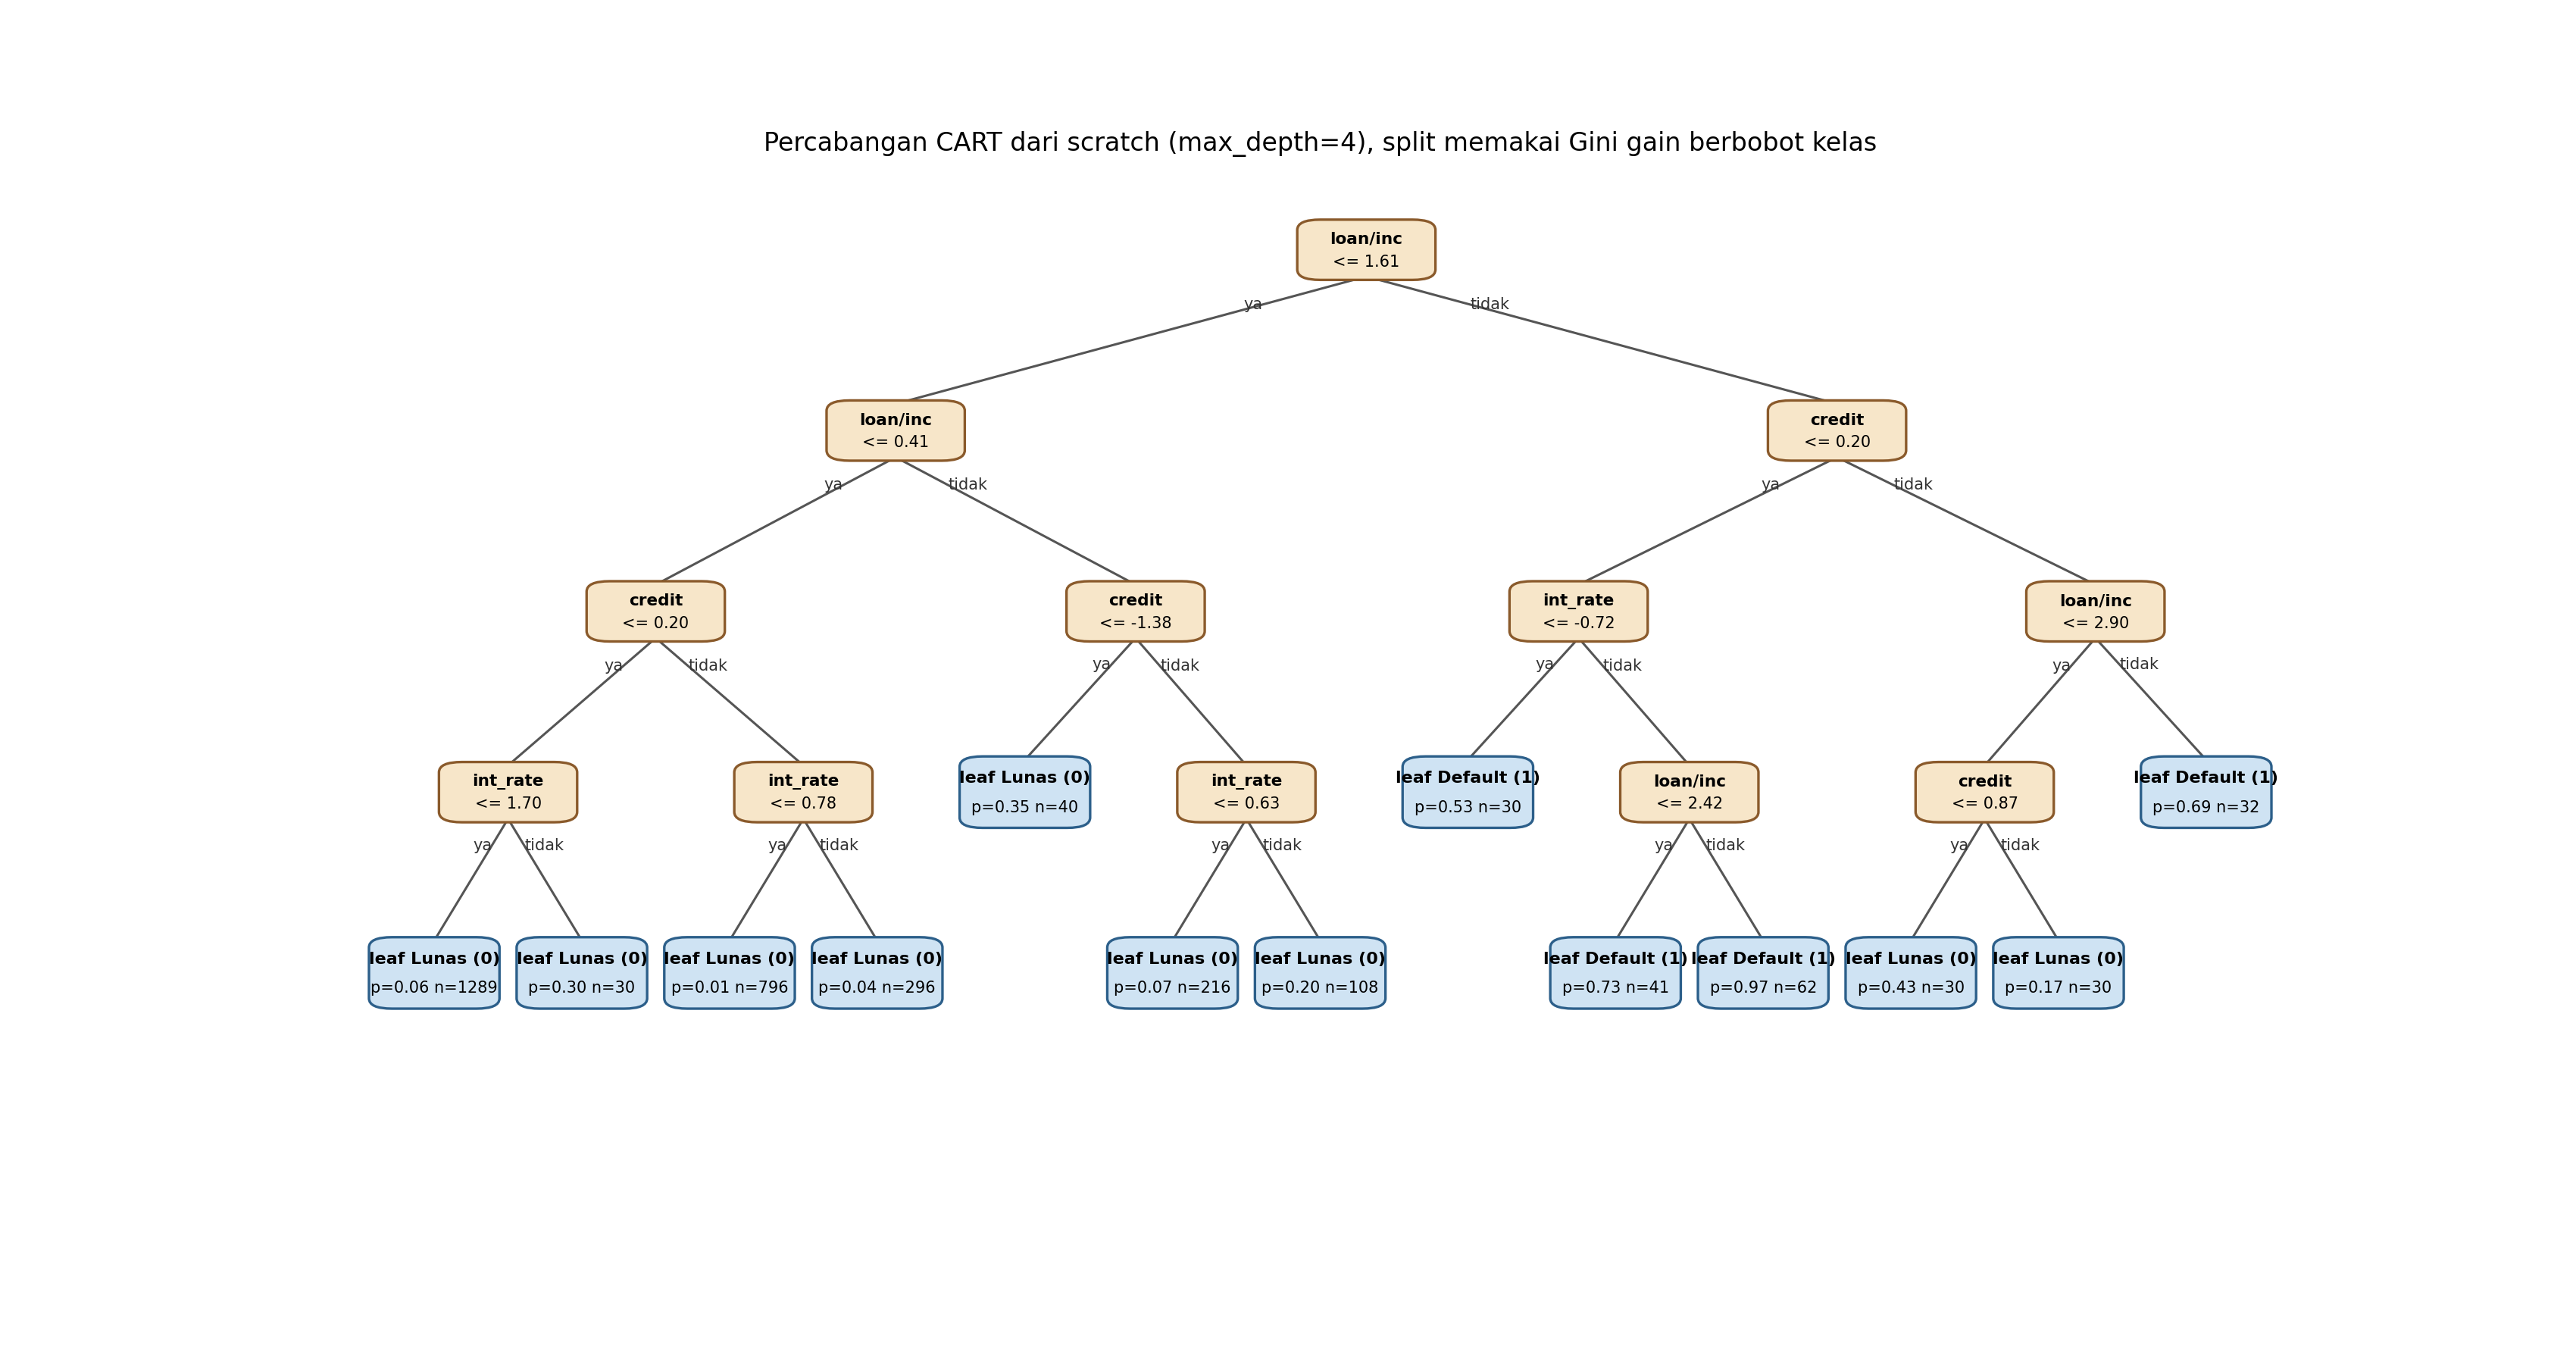
\includegraphics[width=\textwidth]{tree_cart_scratch.png}
\caption{Percabangan CART dari scratch, split memakai Gini gain, leaf berisi probabilitas positif}
\label{fig:tree}
\end{figure}

\subsection{Visualisasi Proses Training Logistic Regression}

Gambar~\ref{fig:lr} menampilkan kontur loss (weighted BCE plus L2) pada dua koefisien model yang dilatih dari nol, dengan lintasan parameter yang dilalui Adam per epoch diwarnai dari epoch awal ke akhir. Titik mulai ada di koordinat nol, lalu lintasan bergerak menuju dasar lembah loss yang diakhiri tanda bintang pada solusi akhir. Gambar ini dibuat dengan mencatat koordinat koefisien di setiap epoch selama training, tanpa mengubah kelas modelnya.

\begin{figure}[h]
\centering
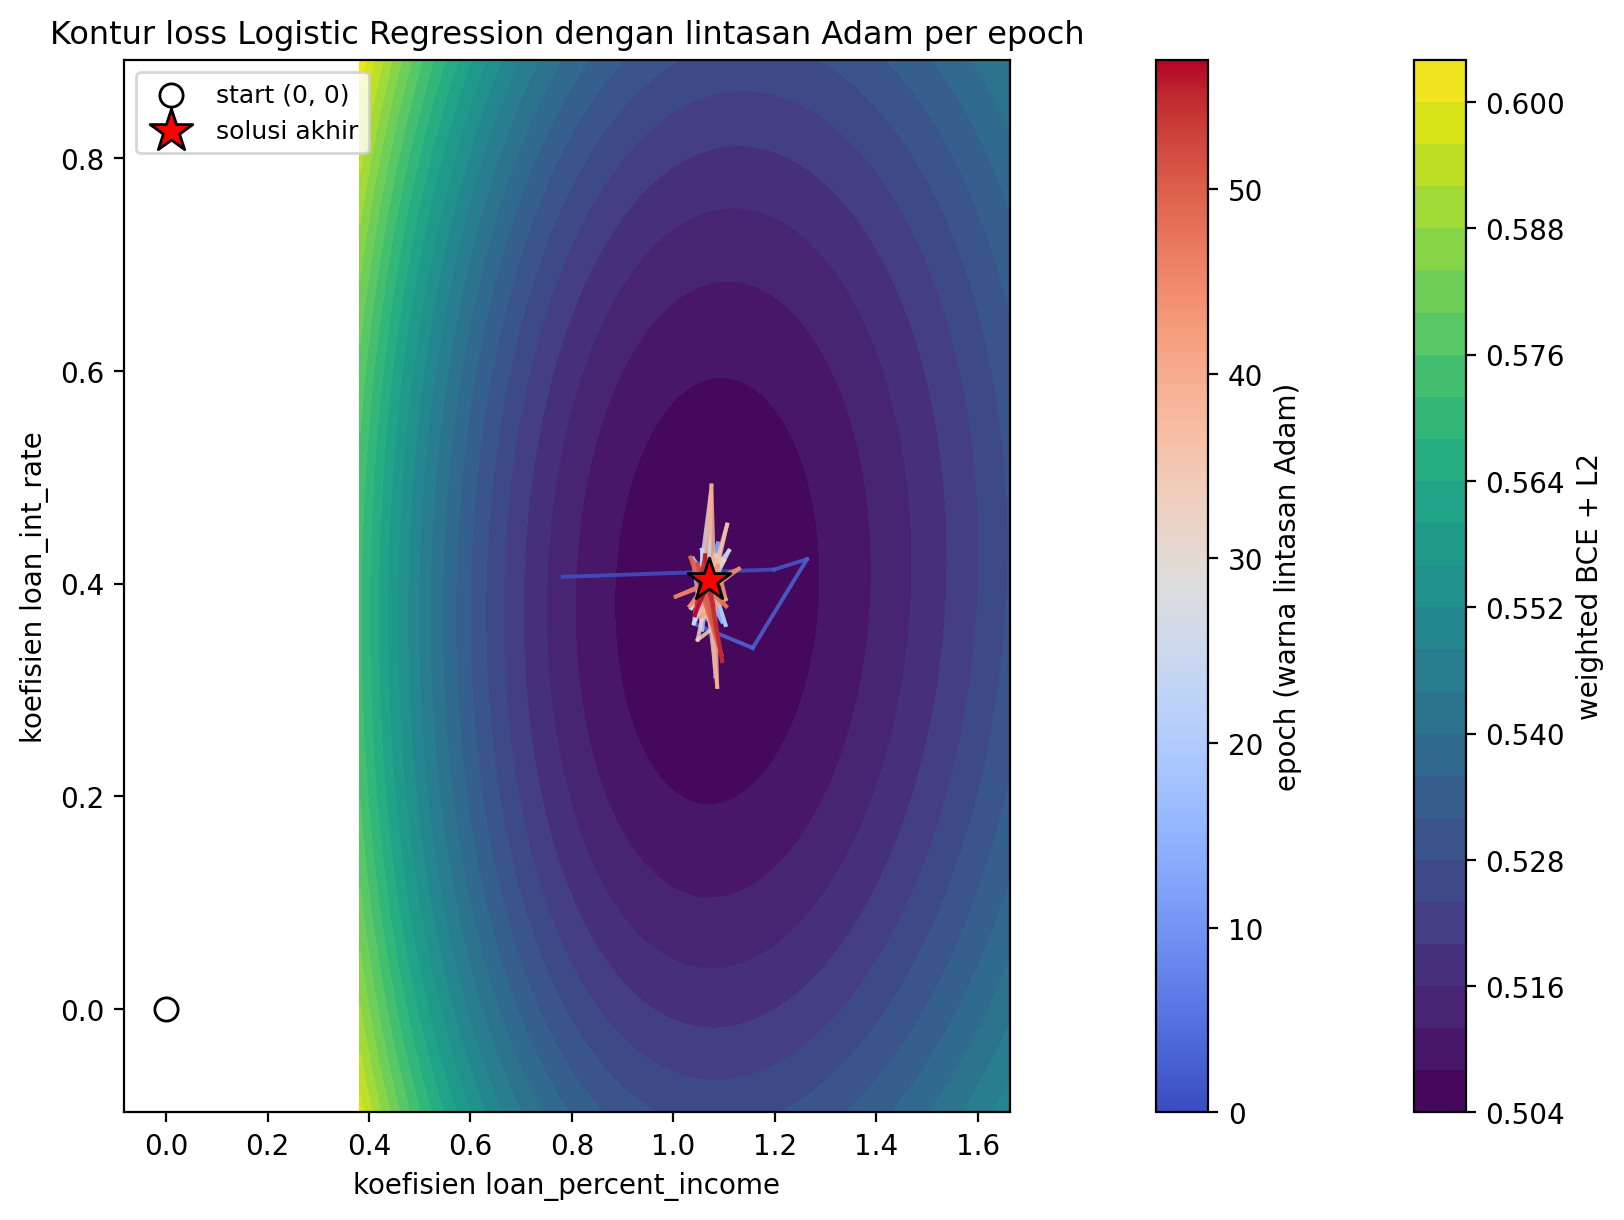
\includegraphics[width=0.72\textwidth]{lr_loss_contour_adam.png}
\caption{Kontur loss Logistic Regression dan lintasan Adam selama training}
\label{fig:lr}
\end{figure}

\FloatBarrier
\section{Referensi}

\begin{enumerate}[label={[\arabic*]}]
\item L. Breiman, J. Friedman, R. Olshen, dan C. Stone. \emph{Classification and Regression Trees}. Wadsworth, 1984.
\item C. M. Bishop. \emph{Pattern Recognition and Machine Learning}. Springer, 2006.
\item T. Hastie, R. Tibshirani, dan J. Friedman. \emph{The Elements of Statistical Learning}, edisi 2. Springer, 2009.
\item C. Cortes dan V. Vapnik. Support-Vector Networks. \emph{Machine Learning} 20(3):273-297, 1995.
\item D. P. Kingma dan J. Ba. Adam: A Method for Stochastic Optimization. \emph{ICLR}, 2015.
\item F. Pedregosa dkk. Scikit-learn: Machine Learning in Python. \emph{JMLR} 12:2825-2830, 2011.
\item Halaman kompetisi \emph{AI Lab Recruitment Task 2}, \url{https://www.kaggle.com/competitions/ai-lab-recruitment-task-2}.
\end{enumerate}

\end{document}
